\chapter{Teorie}
\newacronym{er}{ER}{Entity-Relationship}

V~této kapitole představíme potřebné teoretické koncepty, které bude využívat výsledná aplikace.
Mezi tyto koncepty patří \acrfull{er} model a nově vyvíjený konceptuální model v podobě schematické kategorie~\cite{svoboda_categorical_2021} v rozšířené verzi navržené vedoucím práce.

\section{Entity Relationship}

Datový model \acrfull{er} poprvé představil Peter Pin-Shan Chen už v~roce 1976~\cite{chen_entity-relationship_1976}.
Od té doby se však \acrshort{er} vyvíjel, jak se potřeby datového modelování rozšiřovaly.
\acrshort{er} není standardizováno, ale jednu moderní verzi představili Atzeni, Ceri, Paraboschi a Torlone~\cite[s.~163-179]{atzeni_database_1999}.
Na jejich \acrshort{er} modelu založíme ten náš, který zde popíšeme.

V~Tabulce~\ref{tab:er-constructs} jsou vyobrazeny jednotlivé konstrukty \acrshort{er} modelu.
Zde blíže popíšeme sémantiku jednotlivých konstruktů:
\begin{itemize}
  \item Entitní typ (Entity Type) reprezentuje předpis pro instance entit reálného světa.
        Každý entitní typ má jméno, které je unikátní v daném schématu.
  \item Vztahový typ (Relationship Type) reprezentuje vztah mezi dvěma nebo více (ne nutně různými) entitními typy.
        Každý vztahový typ má jméno.
  \item Atribut (Attribute) reprezentuje vlastnost entitních nebo vztahových typů.
        Každý atribut má jednoznačné jméno.
  \item Složený atribut (Composite Attribute) je atribut, který má sám atributy.
        Zakazujeme však další větvení, tedy atributy složeného atributu už samy nemohou být složené.
        Každý složený atribut má sám jméno, podobně jako jeho vlastní atributy.
  \item \label{def:cardinality}Kardinalita (Cardinality) je dvojice $(a, b) \in \set{\zero, \one}\times \set{\one, \many}$, kde $a$ nazýváme minimální kardinalita (spodní hranice) a $b$ maximální kardinalita (horní hranice).
        Kardinalitu musí mít všechny atributy a každý účastník vztahového typu.
        Výchozí kardinalita je $(1, 1)$ a ve schématu se většinou neuvádí.
        Spodní hranice 0 znamená, že účast je volitelná; hranice 1 znamená, že účast je povinná.
        Horní hranice 1 znamená, že účast je nejvýše jedna; hranice~\many{} znamená, že účastí je libovolný počet.
        \begin{itemize}
          \item Hranice kardinalit pro jednotlivé účastníky vztahů vyjadřují minimální a resp. maximální počet výskytů jednotlivých instancí účastníků v~tomto vztahu.
          \item Hranice kardinalit u~atributů vyjadřují minimální a resp. maximální počet hodnot atributu, které se vztahují k dané instanci entity/vztahu.
        \end{itemize}
  \item Identifikátor (Identifier) umožňuje jednoznačně rozlišit (identifikovat) instance entitních typů.
        Pro každý entitní typ je povinný alespoň jeden identifikátor, ale může jich být více.
        Každý identifikátor je tvořen buď
        \begin{itemize}
          \item jedním nebo více atributy daného entitního typu; takový identifikátor nazýváme interní, nebo
          \item jedním, nebo více vztahovými typy, jichž se daný entitní typ účastní, případně kombinací s~předchozím; takový identifikátor nazýváme externí.
        \end{itemize}
  \item Zobecnění (generalization), nebo také ISA hierarchie\footnote{ISA z anglického \enquote{is a}, analogicky ke vztahu \enquote{has a}} (ISA hierarchy), vyjadřuje vztah podobný dědičnosti v objektově orientovaném programování.
        Jde o vztah mezi entiním typem $E$ zvaným \emph{rodič} a jedním nebo více \emph{dětmi} $E_1, \dots, E_n$.
        Všechny vlastnosti rodiče (atributy, identifikátory, spojené vztahové typy a další ISA hierarchie) jsou i vlastnosti každého z dětí.
        Každá instance dítěte je také instancí rodiče.
\end{itemize}

Entitní typy, které nemají ani jeden interní identifikátor (musí mít tedy externí), nazýváme \emph{slabé} entitní typy (weak entity types).
Pokud mají interní identifikátor, nazýváme je \emph{silné} entitní typy (strong entity types).

Jednoho vztahového typy se může účastnit nejvýše jeden slabý entitní typ, protože pro dva takové by byla identifikace nesmyslná.
Externí identifikace se však může řetězit, jako na Obrázku~\ref{fig:er-external-identifier-chain}.
Nesmí ovšem vzniknout orientovaný cyklus, a to ani v kombinaci s ISA hierarchiemi.
Formálněji -- pokud vytvoříme orientovaný graf $G=(V,E)$ takový, že
\begin{itemize}
  \item vrcholy $V$ jsou entitní typy a
  \item hrany $E$ se skládají z
        \begin{itemize}
          \item pro externí identifikátory orientované hrany od identifikovaného k identifikujícímu entitnímu typu,
          \item pro ISA hierarchii pro každý vztah rodič-dítě, kde $a$ je dítě a $b$ je rodič, orientovanou hranu $(a, b)$,
        \end{itemize}
\end{itemize}
pak graf $G$ musí být acyklický.

Entitní typ, který má externí identifikátor, musí být účastněn vztahového typu (jímž je identifikován) s kardinalitou $(\one,\one)$.
To proto, že když je instance entity identifikována vztahovým typem, musí tento vztah být jednoznačný -- právě jeden.

\begin{figure}[!htb]
  \centering
\includegraphics[width=\maxwidth{\textwidth}]{../img/er-model/external-id-chain.pdf}
  \caption{Zřetězení externích identifikátorů}
  \label{fig:er-external-identifier-chain}
\end{figure}

U~kardinality poznamenejme, že se v~\acrshort{er} modelu často dovoluje použít jako hranice libovolná nezáporná celá čísla, tedy $(a, b)\in \mathbb N_0\times \left(\mathbb N_0 \cup \set{\many}\right)$, tž.~$a\leq b$ (dodefinujeme $\forall a\in\mathbb N_0\colon a < \many$).
Dají se tak vyjádřit přesnější omezení, např. že jeden uživatel může mít maximálně 5 bankovních účtů.
Ovšem námi definované hranice kardinality vyjadřují volitelnost/povinnost pro spodní hranici a jednočetnost/mnohočetnost pro horní hranici.
Pokryjeme jimi z teoretického pohledu a s ohledem na povahu konstruktů v nejrůznějších logických modelech všechny strukturálně odlišné situace, které by mohly nastat.

Dále upozorněme, že místo~\many{} se v~\acrshort{er} modelu může použít symbol \texttt{n} nebo \texttt{N} pro vyjádření \enquote{libovolného počtu}.
Důležitá je ale konzistentnost, aby se v~jednom modelu nevyskytovaly dva různé symboly, což by mohlo zmást čtenáře.
V~této práci budeme používat pouze symbol~\many{}.

\begin{table}[!htb]
  \centering
  \begin{tabular}{@{}rm{7cm}@{}} \toprule
    Konstrukt             & Vizuální reprezentace                                     \\ \midrule
    Entitní typ           & {\centering\includegraphics{../img/er-model/entity.pdf}}  \\
    Vztahový typ          & \includegraphics{../img/er-model/relationship.pdf}        \\
    Atribut               & \includegraphics{../img/er-model/attribute.pdf}           \\
    Složený atribut       & \includegraphics{../img/er-model/composite-attribute.pdf} \\
    Interní identifikátor & \includegraphics{../img/er-model/identifier.pdf}          \\
    Externí identifikátor & \includegraphics{../img/er-model/external-identifier.pdf} \\
    Zobecnění             & \includegraphics{../img/er-model/generalization.pdf}      \\ \bottomrule
  \end{tabular}
  \caption[Grafická reprezentace konstruktů \acrshort{er} modelu]{Grafická reprezentace konstruktů \acrshort{er} modelu, upraveno a přeloženo~\cite[s.~164]{atzeni_database_1999}}
  \label{tab:er-constructs}
\end{table}

\section{Schematická kategorie}

Nejdříve popíšeme kategorii z~teorie kategorií, na níž je schematická kategorie založena.

Kategorie je matematická struktura, která zobecňuje ostatní struktury.
Umožňuje mimo jiné studovat vztahy mezi nimi.
Poprvé byla představena Eilenbergem a MacLanem v~roce 1945~\cite{eilenberg_1945}.

Kategorie $C=(\mathcal O, \mathcal M, \circ)$ se skládá
z~\begin{itemize}
  \item třídy objektů $\mathcal O$,
  \item třídy morfismů $\mathcal M$; každý morfismus $f \in \mathcal M$ má zdrojový objekt $A\in\mathcal O$, cílový objekt $B\in\mathcal O$ a zapisujeme $f: A\to B$ ($f$ je morfismus z~$A$ do $B$),
  \item operace skládání $\circ\colon \mathcal M\times\mathcal M \to \mathcal M$; pro každé dva morfismy $f\in\mathcal M\colon A\to B, g\in\mathcal M\colon B\to C$ musí $g\circ f\in \mathcal M$ (tranzitivita); pro tuto operaci navíc platí axiomy:
        \begin{itemize}
          \item asociativita -- pro morfismy $f\in\mathcal M\colon A\to B, g\in\mathcal M\colon B\to C, h\in\mathcal M\colon C\to D$ platí $h\circ (g \circ f) = (h\circ g)\circ f$,
          \item identita -- pro každý morfismus $f\in\mathcal M\colon A\to B$ a jeho objekty $A, B\in\mathcal O$ existují morfismy $1_A, 1_B\in\mathcal M$, tž. $f\circ 1_A = f = 1_B\circ f$; morfismy $1_A, 1_B$ nazýváme identitami.
        \end{itemize}
\end{itemize}

Kategorie je možné vizuálně reprezentovat orientovaným multigrafem, kde vrcholy jsou objekty a hrany morfismy.
Příklad této vizualizace je na Obrázku~\ref{fig:category-example}.
Jedná se o~kategorii se čtyřmi objekty $A, B, C, D$.

\begin{figure}[!htb]
  \shorthandoff{"}
  \centering
% https://tikzcd.yichuanshen.de/#N4Igdg9gJgpgziAXAbVABwnAlgFyxMJZABgBpiBdUkANwEMAbAVxiRAEEQBfU9TXfIRQBGclVqMWbAELdeIDNjwEio4ePrNWiEAGFu4mFADm8IqABmAJwgBbJGRA4ISURK1sLcyzfuI3zkgATNSaUjrG3iDWdg7UgYgh7uEgxgA6aQDGWFaZAARe1Ax0AEYwDAAK-MpCIFZYxgAWOFExfo4JjgwQEGhEQQDsZBaMcDDixWWV1YJs9U0toZLaIMIA+pw8PrH+8S67IN29RACcw6PjRaXlVUqzOvPNIEseOuuyW9G+wXs-hz19FBnUgjBhjCbXaZ3FQPBpPF4pdb6LgULhAA
\begin{tikzcd}
A \arrow[r, "f"] \arrow[rd, "g\circ f"'] \arrow["1_A"', loop, distance=2em, in=215, out=145] & B \arrow[d, "g"] \arrow["1_B"', loop, distance=2em, in=35, out=325] \\
                                                                                             & C \arrow["1_C"', loop, distance=2em, in=35, out=325]               
\end{tikzcd}
\caption{Příklad kategorie}%
  \label{fig:category-example}%
  \shorthandon{"}
\end{figure}

Schematická kategorie je mechanismus na popis konceptuálního schématu dat založený na teorii kategorií.
Jedná se o~kategorii, jejíž objekty odpovídají jednotlivým entitním typům, atributům a vztahovým typům \acrshort{er} schématu.
Morfismy odpovídají spojením mezi těmito objekty, přičemž aby byly splněny axiomy kategorie, musí se přidat navíc identity a tranzitivní uzávěr těchto morfismů.
Tento koncept společně s~algoritmem převodu z~\acrshort{er} schématu do schematické kategorie uvádí Martin Svoboda, Pavel Čontoš a Irena Holubová~\cite{svoboda_categorical_2021}.
Pro naše účely se v~této práci nebudeme řídit přesně podle této originální publikace, nýbrž schematickou kategorii lehce upravíme.

Schematická kategorie se skládá z~množiny objektů a množiny morfismů.

Objekt je čtveřice (identita, název, data $D$, množina identifikátorů $I$).
Identita je libovolný symbol (např. z~$\mathbb N$), který rozlišuje a unikátně identifikuje všechny objekty, které mají ostatní složky totožné (tedy i pro případ, kdy by všechny ostatní složky byly totožné).
Název reprezentuje textovým řetězcem uživatelské jméno daného objektu.
Data je množina tzv. \emph{properties} a platí $I\subseteq \mathcal P(D)$, tedy je to nadmnožina jednotlivých properties zmíněných v~identifikátorech.
Každý identifikátor sestává z~properties a množina všech identifikátorů je pak množina sestávající z~identifikátorů daného objektu.
Každý objekt musí mít nejméně jeden identifikátor.
Musí platit $D\supseteq \bigcup I$.
Pro ilustraci -- při převodu z~\acrshort{er} bude pro původní entitní typy a atributy platit $D = \bigcup I$, ale u~vztahových typů může být v~$D$ něco navíc.

Morfismus je osmice (signatura, doména, kodoména, směr, název, kardinalita, duplicity, uspořádání).
Signatura vyjadřuje \enquote{cestu}.
Jedná se o~řetězec složený ze signatur jednotlivých morfismů, z~kterých se morfismus skládá.
Pokud se z~dalších morfismů neskládá, je signatura unikátní identitou morfismu (symbol).
Pro ilustraci viz Obrázek~\ref{fig:morphism-signatures}.

Doména a kodoména jsou identity příslušných objektů, odpovídají tak zdrojovému a cílovému objektu kategorie.

Směr udává směr morfismu (který nemusí nutně odpovídat dvojici doména/kodoména).
To proto, že pro každý morfismus bude existovat jeho protějšek.
Směr má dvě možné hodnoty a budeme je značit \one{} (tam), \zero{} (zpět).

Kardinalita odpovídá tomu, jak byla popsána pro \acrshort{er} v~sekci~\ref{def:cardinality}.
Při skládání se kardinality transformují následovně: pro kardinality $(a, b)$ a $(c, d)$ je jejich složením $(\min(a, c), \max(b, d))$.
Uspořádání nad symboly kardinalit je intuitivně $\zero < \one < \many$.

Duplicity a uspořádání jsou booleovské hodnoty (\texttt{true}/\texttt{false}).
Mají význam, pouze pokud je maximální kardinalita~\many.
Říkají, zdali jsou v instanci modelu u objektů spojených daným morfismem povoleny duplicitní objekty, respektive jestli u nich záleží na pořadí.

Morfismy ve schematické kategorii rozdělíme na několik druhů, které jsou všechny vidět na Obrázku~\ref{fig:morphism-signatures}:
\begin{itemize}
  \item \emph{bázové} (base) morfismy jsou ty, které odpovídají jednotlivým spojením a ISA hierarchiím mezi objekty; signatura je identita,
  \item \emph{identitní} (identity) morfismy jsou ty, které vznikly kvůli axiomu identity; signatura je $\varepsilon$,
  \item \emph{odvozené} (derived) morfismy jsou ty, které vznikly kvůli tranzitivitě; signatura je opravdová cesta (zřetězené signatury); zřetězování zapisujeme ve stejném pořadí jako skládání morfismů, aby bylo analogické.
\end{itemize}

\begin{figure}[!htb]
  \centering
  \begin{tikzpicture}
    \tikzset{vertex/.style={shape=circle,draw,minimum size=1em}}
    \tikzset{edge/.style = {->,> = latex'}}
    \node[vertex] (a) {};
    \node[vertex] (b) [right=of a] {};
    \node[vertex] (c) [right=of b] {};

    \draw[edge] (a) to[bend left] node[above] {$13$} (b) ;
    \draw[edge] (b) to[bend left] node[above] {$7$}  (c);
    \draw[edge] (a) to[bend right] node[below] {$7\cdot 13$} (c);
    \draw[edge] (a) to[loop left] node[left] {$\varepsilon$} (a);
    \draw[edge] (b) to[loop above] node[above] {$\varepsilon$} (b);
    \draw[edge] (c) to[loop right] node[right] {$\varepsilon$} (c);
  \end{tikzpicture}
  \caption{Signatury morfismů, $\cdot$ je operace konkatenace (zřetězování) symbolů}
  \label{fig:morphism-signatures}
\end{figure}

% \section{Převod \acrshort{er} na schematickou kategorii}
% 
% \begin{figure}[!htb]
%   \centering
%   \missingfigure{\Huge příklad \acrshort{er} modelu a jeho převodu na schematickou kategorii}
%   \caption{\acrshort{er} model a jeho odpovídající schematická kategorie}
%   \label{fig:test}
% \end{figure}
